%---------------------------------------------------------------------
%
%                          Cap�tulo 2
%
%---------------------------------------------------------------------
\setlength{\parskip}{10pt}
\chapter{Introduction}

\begin{resumen}
	This chapter explains the motivation behind this TFG (Section \ref{cap1:sec:motivation}), the objectives that we set at the beginning of the project (Section \ref{cap1:sec:goals}) and finally , the structure of this memory (Section \ref{cap1:sec:structure}).
\end{resumen}

%------------------------------------------------------------------
\section{Motivation}
%-------------------------------------------------------------------
\label{cap1:sec:motivation}

Some people with cognitive disabilities usually have difficulties when communicating through natural language, and they need to look for alternatives that help them communicate effectively. To help them in communication in some cases pictograms are used, which are graphic symbols representing ideas, objects, actions, etc.

To allow communication through pictograms, communication boards are usually used, which allow to represent messages by means of pictograms on a surface as in Figure \ref{fig:tablerojuguetesen} that shows a board in which the norms of the classroom are indicated. To facilitate the understanding of the boards, templates are usually used. Thus, when viewing the template, users understand the message type faster and understanding is facilitated. Some of the usual formats are the rules boards, the agendas, the calendars, \ldots

%\figura{Bitmap/Capitulo1/JUGUETES}{width=0.5\textwidth}{fig:tablerojuguetesen}{Board that serves to indicate the rules of the classroom.}
\begin{figure}[!ht]
	\centering
	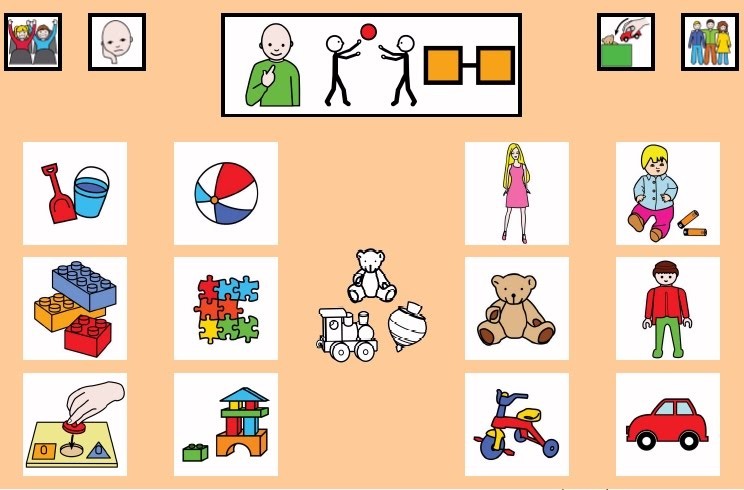
\includegraphics[width=.4\textwidth]{Imagenes/Bitmap/Capitulo1/JUGUETES}
	\caption{Board that serves to indicate the rules of the classroom.}
	\label{fig:tablerojuguetesen}
\end{figure}

Currently, despite the advance of the technologies, in many centers the boards are still created manually with paper, cardboard, cut-outs, stickers, etc. Even for situations in which a board is urgently needed (on a field trip to explain a change of plans, in the supermarket when the child gives a tantrum, in the car to indicate that we are going to take longer than usual, \ldots ) they have to do it with paper and colored pens, since they do not have any tool that allows them to create boards quickly and from any place. When having to perform this task manually, each time a board is created they have to create it from scratch. One way to speed up this task is the use of templates that allow having a fixed structure already created in which you only have to add the specific pictograms of each case to create the board (for example, if we have a template for elections, there would only be to modify the pictograms for the different options of choice). In addition, these templates allow the boards to always have the same format and to make the message faster and more effective.

Despite the multitude of existing tools designed to facilitate the communication of users who use communication boards, it is difficult to find any that fits the formats that the user understands and their needs, which causes the user to be have to adapt to the tools and not vice versa.

For all the reasons mentioned above, there is a need to develop an application that allows users to generate customized templates and boards, without always having to start from scratch or having to adapt to ``universal'' templates that do not correspond to those that use usually. It must be an application that users can access from any device at any time. In this way they will be able to integrate it in their daily life and thus improve the communication of the users who need the communication boards with pictograms to communicate effectively.

%------------------------------------------------------------------
\section{Goals}
%-------------------------------------------------------------------
\label{cap1:sec:goals}

One of the main goals of this work is to develop an application that allows users to generate templates and personalized communication boards based on pictograms, allowing also to be easily reused and speeding up the creation of boards from a template.

In order for the application to have the widest possible range and to adapt to the needs of the users, a user-centered design will be carried out. For this, meetings will be held and evaluations will be carried out with the end users, in order to know the needs they have and to know their opinion about the application and its usability.

We also set ourselves the goal in this work to apply the knowledge acquired during the degree in a project with a social sense and that is also useful beyond being an academic project. Finally, we also set ourselves the goal of acquiring new knowledge that will help us to extend the ones already acquired during the degree.

%------------------------------------------------------------------
\section{Project's Structure}
%-------------------------------------------------------------------
\label{cap1:sec:structure}

This report consists of a total of seven chapters, including this introductory chapter. Below is a brief summary of each of them:

\begin{itemize}
	\item In the \textbf{chapter three} an introduction to the pictograms and their different uses. There is also an analysis of the different pictogram systems and the applications that exist to generate content based on pictograms.
	
	\item  In the \textbf{chapter four} the tools used in the project will be described. Enter \textit{Interact.js}, \textit{html2canvas} and \textit{Realtime Database} from \textit{Firebase}.
	
	\item  In the \textbf{chapter five} will be explained in detail the development of the project, the phase of analysis of requirements, the design of the interface, the implementation of the project, and the evaluations of the users with their results.
	
	\item  In the \textbf{chapter six} and \textbf{chapter seven}, in Spanish and English, the conclusions of the project and future work are presented.
\end{itemize}	


% Variable local para emacs, para  que encuentre el fichero maestro de
% compilaci�n y funcionen mejor algunas teclas r�pidas de AucTeX
%%%
%%% Local Variables:
%%% mode: latex
%%% TeX-master: "../Tesis.tex"
%%% End:
